\documentclass{jsarticle}

\usepackage{url}
\usepackage[dvipdfmx]{graphicx}
\usepackage{amsmath,amsthm,amssymb,ascmac}
\usepackage{fancyhdr}
\usepackage{fancybox}
\usepackage{fancyvrb}

\title{実験1報告書}
\author{小野寺 幸仁}
\date{}

\begin{document}
% タイトルの出力
\maketitle
\clearpage

\section{概要}
近年、計算機性能の向上がリアルタイムなシミュレーションを可能にしつつあり、
仮想現実が身近になり始めている。仮想空間上において、ほかの場所に赴いたり、
空想上の場所で行える体験は楽しく需要も高まっている。

\section{3D酔いについて}

\subsection{概要}
3D酔いとは,普段の感覚とは異なる感覚を引き起こす誘導性の病気の一種で、
別名、「3D酔い」,「シミュレータ病」,「VR酔い」と呼ばれる。これは視覚、バランス感覚、固有感覚、体性感覚の不一致が原因で、人それぞれ強度が異なっている。症状は、失調症、吐き気、眼精疲労などの症状を催す。

\subsection{原因}
3D酔いの原因については速度、視覚の制御、使用時間、高さ、両眼の視差、レイテンシと遅延の6点が挙げられる。
以下にその原因を示す。
\begin{description}
 \item[速度]\mbox{}\\
	     仮想空間での加速度の大きさが3D酔いの発症の速度に正比例しており、加速度の変化が大きいほど、
      3D酔いを引き起こしやすくなる。ただし、等速直線運動の場合は、加速度が0になるため、3D酔いには影響しない.

  \item[視覚の制御]\mbox{}\\
	     ユーザーの頭の動き以外でカメラを動かすことで生じる。
      これは、頭の動きとHMD上の映像が一致していないため、不快感として現れる。
      そこでコントローラでのカメラ視点の変更をできるだけ減らさなければならない

  \item[使用時間]\mbox{}\\
       HMD上の映像を見る時間が長くなるほど、3D酔いが発生しやすくなる。
      この時間は人それぞれ変わるため、15分から30分を使用時間の目安としている。
      しかし、少しでも疲れを感じた場合は、即座にHMDを外さなければならない。

  \item[高さ]\mbox{}\\
       ユーザの仮想空間内での目線の位置のこと。目線の位置が高いのは、体に異常を生じない場合が多いが、
      目線が低い(地面と近い)場合は自分自身の体の認識がずれてしまうのでよろしくない。
      また高低差がある場合は、高低差に従ってカメラの移動を行う。
      例を挙げると、階段を傾斜状に進むのは問題ないが、傾斜を階段状に進むのはよろしくない。

  \item[両眼の視差]\mbox{}\\
       仮想空間での立体視の鍵となっている部分。
      これも個人差があるが、平均的には7cm離れていると仮定されており、Oculus Rift上でも7cmに設定されてある。
      これはアナログ的に変更することが可能だ

  \item[レイテンシと遅延]\mbox{}\\
       現実での動きが、仮想空間では計算機上で処理を行ってからHMD上に表示するため、遅延が発生してしまう。
      なので、計算機上の処理が複雑になるほど、遅延が大きくなる。しかし、
      200msの遅延ならば、体が遅延に慣れてしまい、仮想空間上から戻った際に下船病のような症状を生じてしまうため、気を付けなければならない。
\end{description}

\subsection{対策}
移動は、歩くたびに加速度が生じてしまうのを考慮して、点を移動するテレポートのようなものを用いる。
描画に関しては、計算機の性能を考え処理が大きくなるような空間を作成しない。
また視点変更に関しては、10度ごとなど、固定した数値だけ変更するようにする。
また、花をディスプレイ上に表示することや、歩く際に小さい振動を与えることで、
現実空間の実際に見ている視点に合わせることで小さい改善ができるかもしれない。


\section{Oculus Rift}
\subsection{環境}
\begin{itemize}
  \item CPU
  \item GPU
  \item memory
  \item Oculus Rift CV1
  \item 1
\end{itemize}

\subsection{配線}
\begin{enumerate}
  \item Oculus SensorをUSB3.0につなぐ
  \item Oculus Rift本体のDisplay PortをGPUのDisplay Portにつなぐ
  \item 使う場合は、Xbox OneコントローラをUSBにつなぐ
\end{enumerate}

\subsection{設定}
\begin{enumerate}
  \item
  \item
  \item
  \item
  \item
\end{enumerate}

\subsection{コントローラのボタン設定}
調べたコントローラのボタン設定について図に示す。
これは、正式な変数名になっておりUnity及びC++どちらともで使われる。

\section{Unityでの作成}
\subsection{使用環境とツール}
\begin{itemize}
  \item Unity5.4.0
  \item OculusSmapleFrameWork\_1.16.0
  \item ovr\_unity\_utiilities\_1.16.0
  \item ovr\_avatar\_sdk\_1.16.0
\end{itemize}





\subsection{導入手順}
\begin{enumerate}
  \item unity5.4.0、ovr\_unity\_utilities\_1.16.0、
        OculusSmapleFrameWork\_1.16.0とovr\_avatar\_sdk\_1.16.0のダウンロード
  \item Unity5.4.0でファイルの作成(必要であればProject name,Locationの変更)
  \item UnityにOculusSmapleFrameWork\_1.16.0、ovr\_unity\_utiilities\_1.16.0、ovr\_avatar\_sdk\_1.16.0のインポート
  \item Edit->Project Setting->PlayerのVirtual Reality Supportedにチェック
  \item Virtual Reality SDKsでOculusの選択
\end{enumerate}

\subsection{HMDへの投影}
\begin{enumerate}
  \item HierarchyのMain cameraの削除
  \item assets\textbackslash OVR\textbackslash Prefabs\textbackslash OVRcameraRigをHierarchyに移動する
  \item 画面上部の実行ボタンで投影
\end{enumerate}


\subsection{Oculus Touchのアバター設定}
\begin{enumerate}
  \item Hierarch内でcreate emptyを押してGameObjectの作成
  \item 作成したGameObjectの中にOVRCameraRigとAssets\textbackslash OvrAvatar\textbackslash Content\textbackslash Prefabs\textbackslash LocalAvatarを入れる
  \item 画面上部の実行ボタンで実行
  \item Oculus Touch Controllerをセンサ範囲内で使用する
\end{enumerate}

\subsection{オブジェクトの掴みの実装}
\begin{enumerate}
  \item 掴みたいオブジェクトの作成(Gameobject->3D Object->Cube)
  \item 作成したCubeにOVRGrabbableを追加する
  \item LocalAvatarのcontroller\_left,controller\_rightにそれぞれOVRgrabberを追加
  \item

\end{enumerate}



\section{GLUTを用いて作成}
\subsection{使用環境とツール}
以下のツールを用いて作成した。
\begin{itemize}
  \item Visual Studio 2015
  \item Cmake-3.10.1
  \item freeglut-3.0.0
  \item Lhaplus
\end{itemize}

\subsection{GLUTの導入}
\begin{enumerate}
  \item Cmake-3.10.1とfreeglut-3.0.0とLhaplusのダウンロード
  \item freeglutの圧縮ファイルが.gzのため、Lhaplusを用いて解凍
  \item Cmakeのインストール
  \item Cmakeを実行し、source codeにfreeglut-3.0.0、build the binariesでbuildファイルを参照
  \item Configureの中のSpecify the generator for this projectにVisual Studio 14 2015の選択
  \item Configureボタンを押す()

  \begin{figure}[htbp]
    \centering
    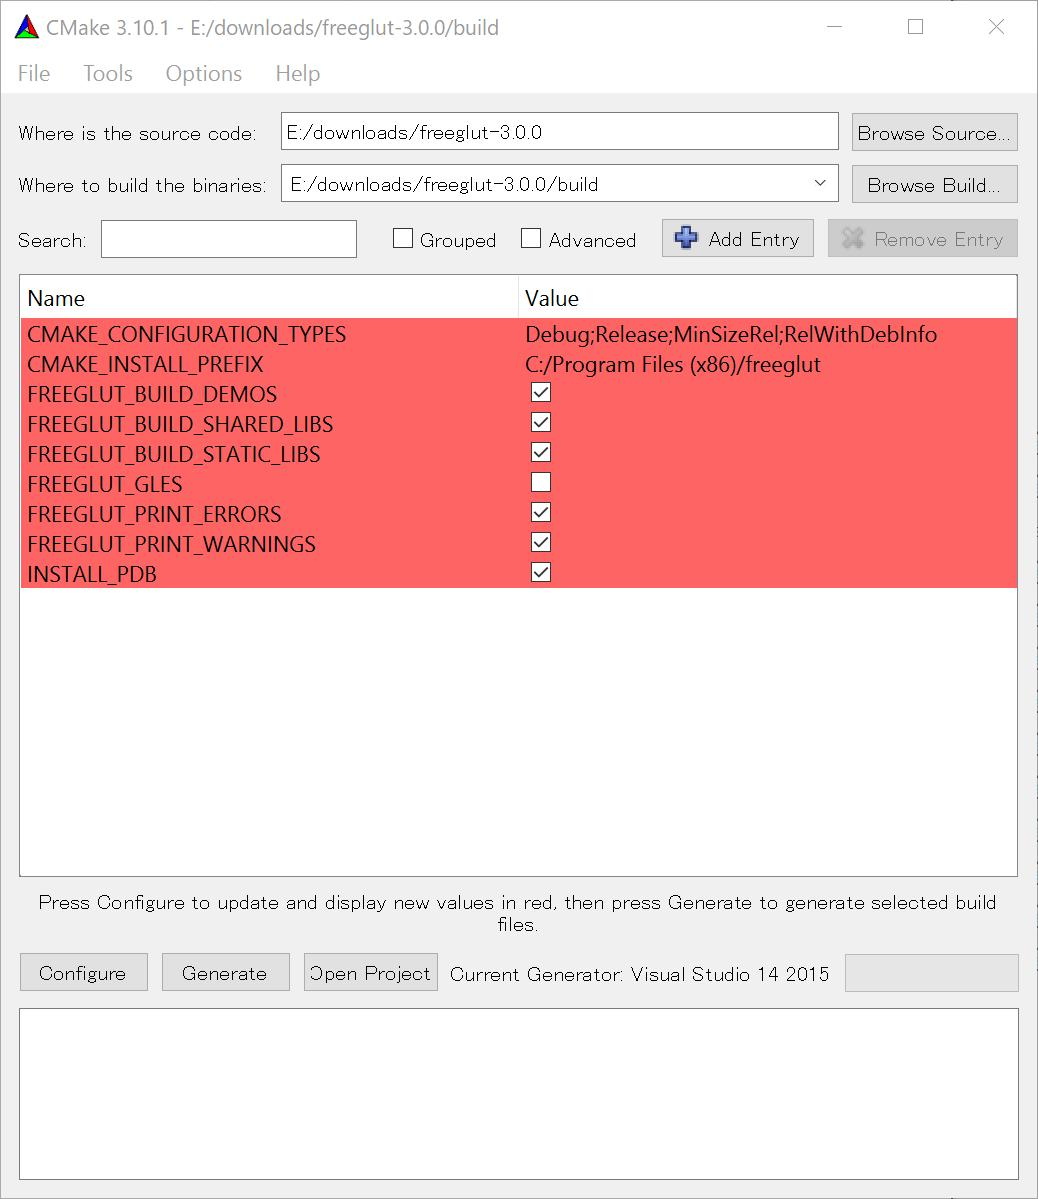
\includegraphics[width=6cm]{Cmake.jpg}
    \caption{CMakeの設定画面}
  \end{figure}

  \item freeglut-3.0.0\textbackslash build\textbackslash freeglut.slnの実行とビルド
  \item freeglutd.lib, freeglut\_staticd.libをC:\textbackslash Program Files (x86)\textbackslash Windows Kits\textbackslash 8.1\textbackslash Lib\textbackslash winv6.3\textbackslash um\textbackslash x86の中へ
  \item freeglutd.dllをC:\textbackslash Windows\textbackslash SysWOW64の中へ
  \item glut.h,freeglut.h,freeglut\_std.h,freeglut\_ext.hをC:\textbackslash Program Files (x86)\textbackslash Windows Kits\textbackslash 8.1\textbackslash Include\textbackslash um\textbackslash glへ
\end{enumerate}

\subsection{2次元空間の作成}
2次元空間で以下のソースコードを作成し、実行の確認を行った。
\begin{itemize}
  \item 空のウィンドウの作成
  \item ウィンドウの出現位置、サイズの変更
  \item 2次元の線を書き、色の変更
  \item マウス、キーボードの使用
\end{itemize}

\begin{figure}[htbp]
 \begin{minipage}{0.5\hsize}
  \begin{center}
   
\includegraphics[width=6cm]{emptyWindow.jpg}
  \end{center}
  \caption{一つめの図}
  \label{fig:one}
 \end{minipage}
 \begin{minipage}{0.5\hsize}
  \begin{center}
   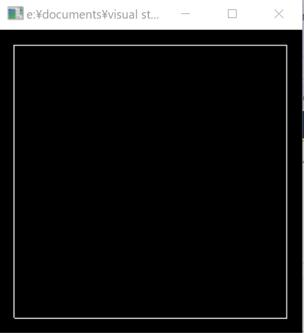
\includegraphics[width=6cm]{whiteSquare.jpg}
  \end{center}
  \caption{二つめの図}
  \label{fig:two}
 \end{minipage}
\end{figure}


\subsection{3次元空間の作成}
3次元空間で以下の実験用のコードを作成し、実行の確認を行った。
\begin{itemize}
  \item 線で立方体の作成
  \item 視点の変更
  \item 面の色付け
  \item アニメーション
  \item ダブルバッファリング
  \item 射影
  \item カリング
\end{itemize}

\begin{figure}[htbp]
  \centering
  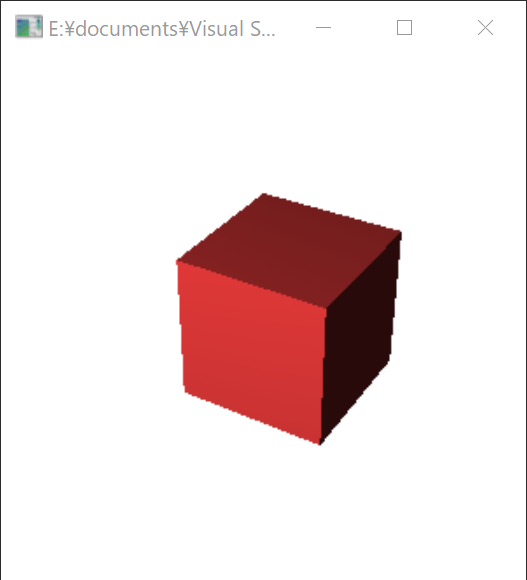
\includegraphics[width=6cm]{3D_Cube.png}
  \caption{立方体の作成}
\end{figure}

\subsection{GLUTを用いてHMD上での投影}
3次元空間をGLUTで作成し、HMD上で投影を試みた。
しかし、投影する際にトラッキングやバッファリング等の設定を行わなければならず、
1からソースコードを書くのは難しい。
そこでOculusSDKよりOculusRoomTiny(GL)の流用を行った。
理由は、すでにHMD上に映すための関数がそろっていたからだ 
そこで、空間を作成している部分をGLUTで作成しなおしてHMD上で確認した。
HMD上の画像をミラーリングしたものを図に示す。
画面が見やすいように立方体のほかに壁も作成した。
基盤となっている部分はすべてサンプルコードを用いたため、Unity同様、3D空間の作成しかしていない。









\end{document}
